\documentclass[12pt,letterpaper]{article}
\usepackage[utf8]{inputenc}
\usepackage{amsmath,amsthm,amsfonts,amssymb,amscd}
\usepackage[table]{xcolor}
\usepackage[margin=2.5cm]{geometry}
\usepackage{ragged2e}
\usepackage{graphicx}
\usepackage{multicol}
%\usepackage[brazil]{babel}
\newlength{\tabcont}
\setlength{\parindent}{0.0in}
\setlength{\parskip}{0.05in}

\begin{document}

	\large \textbf{Nome}: Luís Felipe de Melo Costa Silva \\
	\textbf{Número USP}: 9297961

	\begin{center}
		\LARGE \bf
		Lista de Exercícios 3 - MAC0425
	\end{center}

	\section*{Exercício 10.6}

	Quando os efeitos negativos de uma ação são descartados, nós adicionamos apenas os efeitos positivos, aumentando o conjunto de literais em que podemos encontrar a solução. Nesse caso, estamos simplificando as condições, tornando o problema menos restrito e mais geral, acabando com um problema mais fácil do que o original.

	\section*{Exercício 10.9}

	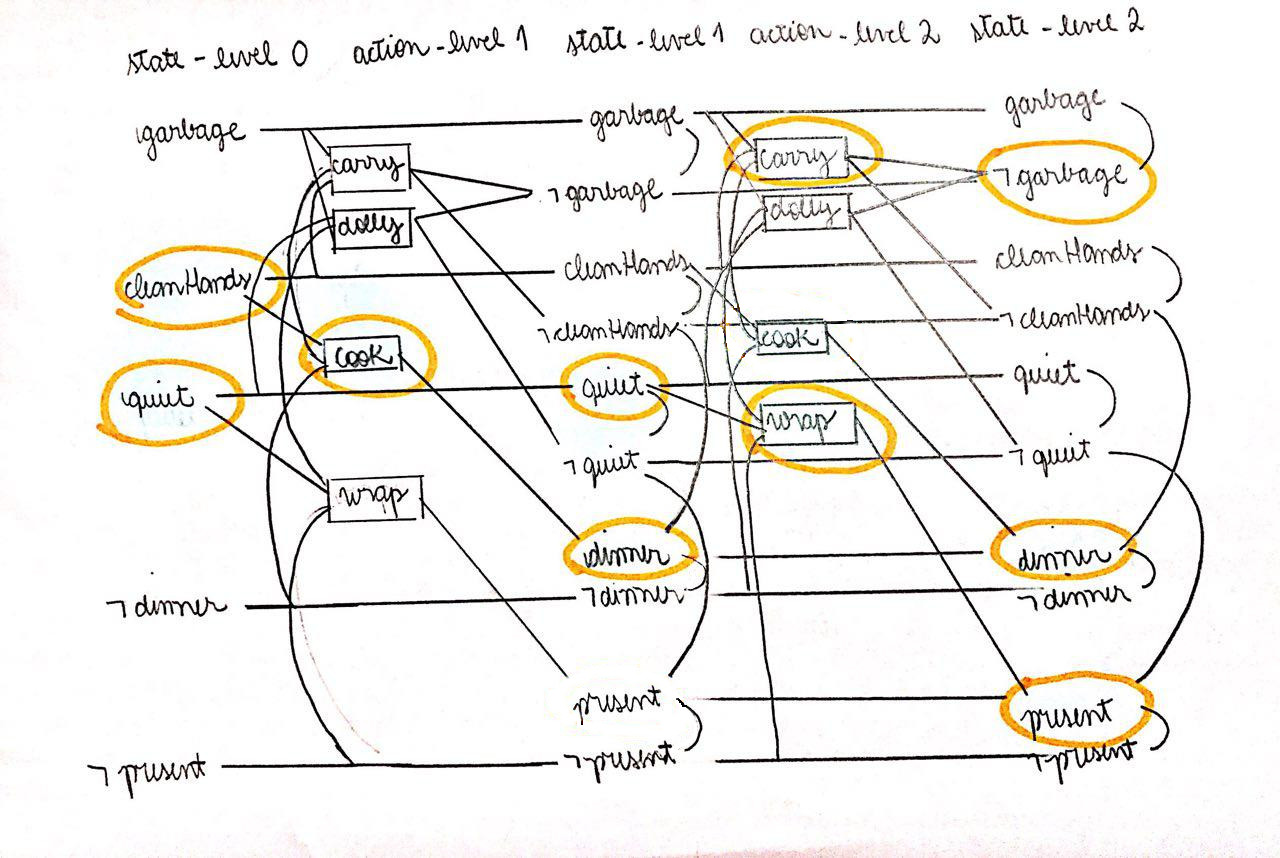
\includegraphics[width=\textwidth]{graphplan.jpg}

	Começamos o Graphplan com os sequentes literais e os que não temos da meta no \textit{state-level 0}.
	
	Então, aplicamos as ações possíveis a partir desses literais em \textit{action-level 1}. Podemos observar os seguintes mutexes:

	\begin{itemize}
		\item Por interferência:
		\begin{itemize}
			\item \textit{carry} e \textit{cook}
			\item \textit{dolly} e \textit{wrap}
		\end{itemize}
		\item Por efeitos inconsistentes:
		\begin{itemize}
			\item \textit{carry} e manutenção de \textit{garbage}
			\item \textit{carry} e manutenção de \textit{cleanHands}
			\item \textit{dolly} e manutenção de \textit{garbage}
			\item \textit{dolly} e manutenção de \textit{quiet}
			\item \textit{cook} e manutenção de \textit{$\lnot$dinner}
			\item \textit{wrap} e manutenção de \textit{$\lnot$present}
		\end{itemize}
	\end{itemize}
	
	
	Chegamos ao \textit{state-level 1}, e temos os seguintes mutexes:

	\begin{itemize}
		\item Por suporte inconsistente:
		\begin{itemize}
			\item \textit{garbage} e \textit{$\lnot$garbage}
			\item \textit{cleanHands} e \textit{$\lnot$cleanHands}
			\item \textit{quiet} e \textit{$\lnot$quiet}
			\item \textit{dinner} e \textit{$\lnot$dinner}
			\item \textit{present} e \textit{$\lnot$present}
		\end{itemize}
		\item Por efeitos que competem
		\begin{itemize}
			\item \textit{$\lnot$quiet} e \textit{present}
			\item \textit{garbage} e \textit{$\lnot$cleanHands}
			\item \textit{garbage} e \textit{$\lnot$quiet}
			\item \textit{$\lnot$cleanHands} e \textit{dinner}
		\end{itemize}
	\end{itemize}
	
	Prosseguimos para o \textit{action-level 2}, e pode-se observar os mutexes:

	\begin{itemize}
		\item Por interferência e efeitos inconsistentes:
		\begin{itemize}
			\item manutenção de \textit{garbage} e manutenção de \textit{$\lnot$garbage}
			\item manutenção de \textit{cleanHands} e manutenção de \textit{$\lnot$cleanHands}
			\item manutenção de \textit{quiet} e manutenção de \textit{$\lnot$quiet}
			\item manutenção de \textit{dinner} e manutenção de \textit{$\lnot$dinner}
			\item manutenção de \textit{present} e manutenção de \textit{$\lnot$present}
		\end{itemize}
		\item Por interferência:
		\begin{itemize}
			\item \textit{carry} e \textit{cook}
			\item \textit{dolly} e \textit{wrap}
		\end{itemize}
		\item Por efeitos inconsistentes:
		\begin{itemize}
			\item \textit{carry} e manutenção de \textit{garbage}
			\item \textit{carry} e manutenção de \textit{cleanHands}
			\item \textit{dolly} e manutenção de \textit{garbage}
			\item \textit{dolly} e manutenção de \textit{quiet}
			\item \textit{cook} e manutenção de \textit{$\lnot$dinner}
			\item \textit{wrap} e manutenção de \textit{$\lnot$present}
		\end{itemize}
		\item Por necessidades que competem:
		\begin{itemize}
			\item \textit{cook} e manutenção de \textit{$\lnot$cleanHands}
			\item \textit{wrap} e manutenção de \textit{$\lnot$quiet}
		\end{itemize}
	\end{itemize}

	Por fim, temos o \textit{state-level 2}, que nos dá os seguintes mutexes:

	\begin{itemize}
		\item Por suporte inconsistente:
		\begin{itemize}
			\item \textit{garbage} e \textit{$\lnot$garbage}
			\item \textit{cleanHands} e \textit{$\lnot$cleanHands}
			\item \textit{quiet} e \textit{$\lnot$quiet}
			\item \textit{dinner} e \textit{$\lnot$dinner}
			\item \textit{present} e \textit{$\lnot$present}
		\end{itemize}
		\item Por efeitos que competem
		 \begin{itemize}
			\item \textit{$\lnot$quiet} e \textit{present}
			\item \textit{garbage} e \textit{$\lnot$cleanHands}
			\item \textit{garbage} e \textit{$\lnot$quiet}
			\item \textit{$\lnot$cleanHands} e \textit{dinner}
		\end{itemize}
	\end{itemize}


	Para encontrarmos o plano para resolver esse problema, começamos selecionando os literais da meta em \textit{state-level 2}. Então, pegamos ações no \textit{action-level 2} que não estão em mutex entre si (\textit{carry, wrap}) e as pré-condições dessas ações (\textit{quiet}) e a ação de manutenção dos literais que não foram contemplados com as ações escolhidas (\textit{dinner}), que estão no \textit{state-level 1}. Olhamos para o \textit{action-level 1} e procuramos as ações que geram \textit{dinner} e \textit{quiet}. A ação \textit{cook} gera \textit{dinner}, e \textit{quiet} é gerado por uma ação de manutenção. Logo, nosso plano é [\textit{cook, carry, wrap}]. Existem outros planos possíveis, por exemplo: [\textit{wrap, cook, dolly}].    

	\section*{Exercício MDP}
	
	Usando a definição de que MDP é uma tupla $<S, D, A, T, R>$ do slide 3 da segunda aula de Planejamento Probabilístico, usaremos a seguinte fórmula para calcular $V^n$ (do slide 14 da mesma aula):
	
	\begin{center}
		$V^n(s) = R(s) + max_{a \in A}({\sum_{s \in S}T(s, a, s')\cdot V^{n-1}(s')})$
	\end{center}
	
	Começamos com $V^0(s) = R(s), \forall s \in S$. Então, teremos:
	
	\begin{itemize}
		\item Para n = 1
		\begin{itemize}
			\item $V^1(s1) = 0 + max(V^0(s2);0,5\cdot V^0(s1) + 0,5\cdot V^0(s4)) \\= max(0;0,5\cdot 0 + 0,5\cdot 100) = 50$
			\item $V^1(s2) = 0 + max(0,8\cdot V^0(s3) + 0,2\cdot V^0(s5)) \\= max(0,8\cdot 0 + 0,2\cdot (-100)) = -20$
			\item $V^1(s3) = 0 + max(V^0(s2);V^0(s4)) \\= max(0; 100) = 100$
			\item $V^1(s4) = 100 + max(V^0(s1);V^0(s3);V^0(s5)) \\= 100 + max(0;0;-100)) = 100$
			\item $V^1(s5) = -100 + max(V^0(s2);V^0(s4)) \\= -100 + max(0;100) = 0$
		\end{itemize}
		\item Para n = 2
		\begin{itemize}
			\item $V^2(s1) = 0 + max(V^1(s2);0,5\cdot V^1(s1) + 0,5\cdot V^1(s4)) \\= max(-20;0,5\cdot 50 + 0,5\cdot 100) = 75$
			\item $V^2(s2) = 0 + max(0,8\cdot V^1(s3) + 0,2\cdot V^1(s5)) \\= max(0,8\cdot 100 + 0,2\cdot 0) = 80$
			\item $V^2(s3) = 0 + max(V^1(s2);V^1(s4)) \\= max(-20; 100) = 100$
			\item $V^2(s4) = 100 + max(V^1(s1);V^1(s3);V^1(s5)) \\= 100 + max(50;100;0)) = 200$
			\item $V^2(s5) = -100 + max(V^1(s2);V^1(s4)) \\= -100 + max(-20;100) = 0$
		\end{itemize}
		\item Para n = 3
		\begin{itemize}
			\item $V^3(s1) = 0 + max(V^2(s2);0,5\cdot V^2(s1) + 0,5\cdot V^2(s4)) \\= max(80;0,5\cdot 75 + 0,5\cdot 200) = 137,5$
			\item $V^3(s2) = 0 + max(0,8\cdot V^2(s3) + 0,2\cdot V^2(s5)) \\= max(0,8\cdot 100 + 0,2\cdot 0) = 80$
			\item $V^3(s3) = 0 + max(V^2(s2);V^2(s4)) \\= max(80; 200) = 200$
			\item $V^3(s4) = 100 + max(V^2(s1);V^2(s3);V^2(s5)) \\= 100 + max(75;100;0)) = 200$
			\item $V^3(s5) = -100 + max(V^2(s2);V^2(s4)) \\= -100 + max(80;200) = 100$
		\end{itemize}
	\end{itemize}
	
	As tabelas $V$ e $\pi$ ficam assim:
	
	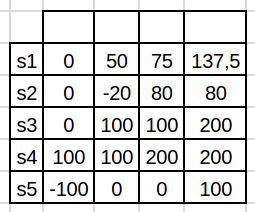
\includegraphics[width=4cm]{tabelav.png}
	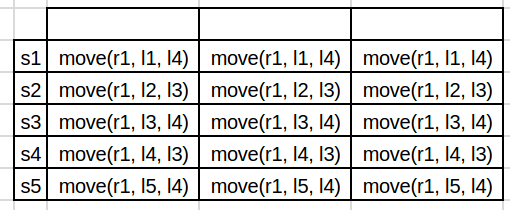
\includegraphics[width=7.5cm]{tabelapi.png}

	\section*{Exercício Q-Learning}
	
	Para esse exercício vamos usar a fórmula do \textit{Q-value update}, que consiste em:
	
	\begin{center}
		$Q(s,a) \leftarrow (1-\alpha)\cdot Q(s,a) + \alpha(r+\gamma\cdot max_{a'\in A}Q(s',a'))$
	\end{center}
	
	O enunciado nos pede para usar $\alpha = 1$ e $\gamma = 0,9$. Com esses valores, nossa fórmula ficará: 
	
	\begin{center}
		$Q(s,a) \leftarrow (r+0,9\cdot max_{a'\in A}Q(s',a'))$
	\end{center}
	
	Começando com a tabela zerada e fazendo os cálculos para os episódios pedidos, teremos:
	
	\textbf{1.}
	
	$Q(3,S) = -10 + 0,9 \cdot 0 = -10$\\
	$Q(3,N) = 0 + 0,9 \cdot 0 = 0$\\
	$Q(1,N) = -10 + 0,9 \cdot 0 = -10$\\
	$Q(1,O) = 10 + 0,9 \cdot 0 = 10$\\
	
	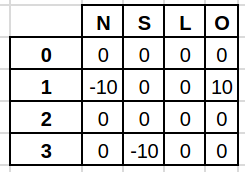
\includegraphics[width=4cm]{tabelaexperiencia1.png}
	
	\textbf{2.}
	
	$Q(2,L) = 0 + 0,9 \cdot 0 = 0$\\
	$Q(3,N) = 0 + 0,9 \cdot 0 = 0$\\
	$Q(1,N) = -10 + 0,9 \cdot 0 = -10$\\
	$Q(1,L) = -10 + 0,9 \cdot 0 = -10$\\	
	$Q(1,O) = 10 + 0,9 \cdot 0 = 10$\\
	
	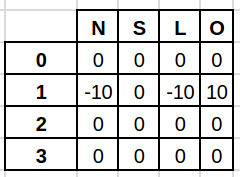
\includegraphics[width=4cm]{tabelaexperiencia2.png}
	
\end{document}
